\documentclass[11pt]{article}
\usepackage{amsmath,amssymb,amsthm}
\usepackage{graphicx}
\usepackage[margin=1in]{geometry}
\usepackage{fancyhdr}
\usepackage{tkz-berge}
\usetikzlibrary{positioning,chains,fit,shapes,calc}
\setlength{\parindent}{0pt}
\setlength{\parskip}{5pt plus 1pt}
\setlength{\headheight}{13.6pt}
\newcommand\question[2]{\vspace{.25in}\hrule\textbf{#1: #2}\vspace{.5em}\hrule\vspace{.10in}}
\renewcommand\part[1]{\vspace{.10in}\textbf{(#1)}}
\newcommand\algorithm{\vspace{.10in}\textbf{Algorithm: }}
\newcommand\correctness{\vspace{.10in}\textbf{Correctness: }}
\newcommand\runtime{\vspace{.10in}\textbf{Running time: }}
\pagestyle{fancyplain}
\lhead{\textbf{\NAME\ (\UID)}}
\chead{\textbf{HW\HWNUM}}
\rhead{ECE 6810, \today}
\begin{document}\raggedright
%Section A==============Change the values below to match your information==================
\newcommand\NAME{Vikas Kumar Rao}  % your name
\newcommand\UID{U1072596}     % your utah UID
\newcommand\HWNUM{2}              % the homework number
%Section B==============Put your answers to the questions below here=======================
% no need to restate the problem --- the graders know which problem is which,
% but replacing "The First Problem" with a short phrase will help you remember
% which problem this is when you read over your homeworks to study.
\question{1}{Pipelining performance}
\part{a}
Given - 
Cycle Time (CT) = 10ns\\
Instruction Count (IC) = 1000\\
cycles per instruction (CPI) = 1\\

$CPU_{time} = CT \times CPI \times IC = 10ns \times 1000 \times \1 = 10000ns$\\

\part{b}

We know that speedup is given

$speedup = \frac{\text{CPU Time}_{old}}{\text{CPU Time}_{new}}$

For a perfect partitioning and pipelining, a 10 stage pipeline and 1000 instructions will require 1009 pipelined register stages. Since 1 instruction takes 1ns in each pipelined stage, we will have 1009 x 1ns delay in pipelined stages.
Since there is a 1ns delay for every pipelined stage register, we will have 1008 x 1ns registered pipeline delays. Since there are 2 bubbles(stalls) every 10 cycles, we have 1000/10 = 100 cycles of branch instructions, hence 100 X 2ns = 200 ns.

$\text{CPU Time}_{new} = (1009 + 1008 + 200)ns = 2217ns$

$speedup = \frac{10000ns}{2217ns} = 4.51$

\question{2}{Control hazards}

a) Given that 20\% of the instructions are branched, 80\% are non branching instructions which take 1 cycle time to complete.\\
b) In the branching instruction of 20\%, there are two cases - 60\% cases taken and 40\% not taken. Assuming each branch instruction computation takes 1 cycle for execution.
  1) Since the 2 stall cycles in case of taken branches can be utilized, the taken part branches take just 1 cycle for execution.
  2) Since the 2 stall cycles in case of not taken branches cannot be utilized, the 2 stall cycles add upto branch execution cycles, which effectively becomes 3.

Thus, cycles per instruction is given as -
$CPI = 0.8*1 + 0.2*(0.6*1 + 0.4*3) = 1.16$ 

\question{3}{Multi-cycle instructions}

\part{a}{timing diagram}\\
The timing diagram with no ALU forwarding is as shown below ~\ref{no_fwd}. The assumptions made here are that there is no ALU forwarding allowed and hence, RR in 3rd instruction has to wait until data is available at F2 after LOAD. similarly, DIV instruction RR has to wait until F0 data is available from MUL.

Table notations - CC - clock cycle.
\begin{figure}[ht]
	\begin{center}
	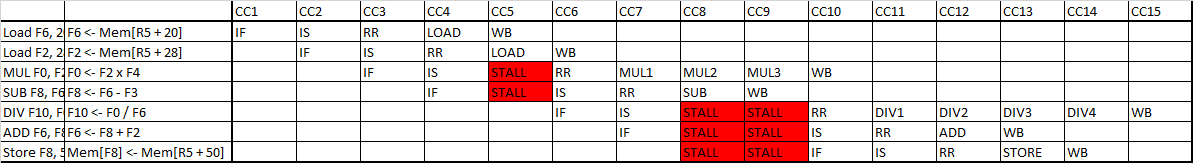
\includegraphics[scale = 0.60]{no_fwd}
	\end{center}
	\vspace{-4ex}
	\caption{timing diagram with no ALU forward}
	\label{no_fwd}
	\vspace{-3ex}
\end{figure}


The timing diagram with ALU forwarding is as shown below ~\ref{alu_fwd}. The assumption made here is that the RR in 3rd instruction can read any stale value, but since ALU can do forwarding, it will overwrite the data from LOAD-F2 to MUL1-F2. Similarly, data from MUL3-F0 will overwrite DIV1-F0 with aLU forwarding and hence we need just one STALL cycle.
\begin{figure}[ht]
	\begin{center}
	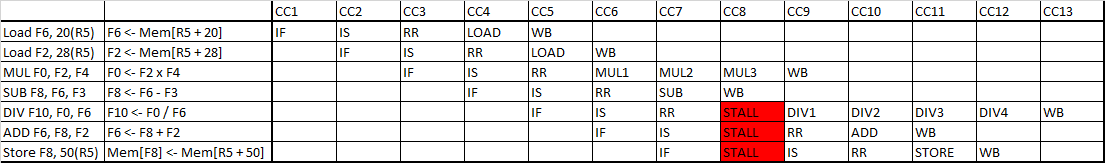
\includegraphics[scale = 0.60]{alu_fwd}
	\end{center}
	\vspace{-4ex}
	\caption{timing diagram with ALU forwarding}
	\label{alu_fwd}
	\vspace{-3ex}
\end{figure}

\part{b}{structural and data hazards}\\
Just by looking at the code there are 6 potential data hazards, they are all of the kind Read after Write(RAW).\\
a) For register F6 between 1st Load and SUB\\
b) For register F6 between 1st Load and DIV\\
c) For register F2 between 2nd Load and MUL\\
d) For register F2 between 2nd Load and ADD\\
e) For register F0 between MUL and DIV\\
f) For register F8 between SUB and ADD\\
But after drawing the timing diagram with appropriate stalls we can see that only data hazard due to RAW for case c) and e) with respect to table ~\ref{no_fwd} needs fixing. In case of table ~\ref{alu_fwd}, only case e) is the visible data hazard.

There are no structural hazards with respect to timing diagram.

\question{4}{Points of production and consumption}
\part{a}{throughput of un-pipelined processor}\\
For the un-pipelined processor, the dependencies doesn't matter as every new instruction after completing the entire computation, hence the time taken is given as  - $(36+0.5)ns = 36.5ns$

Throughput = $\frac{1}{36.5ns} = 0.027\times 10^9 \text{instructions per second}$

\part{b}{throughput of 12 stage pipelined processor}\\

In the 12 stage pipeline, every individual stage time is given as $\frac{\text{execution time}}{\text{number of stages}} = \frac{36ns}{12} = 3ns$.
Each stage has $0.5ns$ of latch delay, and hence the total delay between each stage is $3.5ns$. 

Dependent instruction stages are computed as - $\frac{POP-POC}{\text{individual pipeline stage time}}=\frac{12ns}{3ns}=4$

Dependent instruction delay is given as - $(POP-POC)+(\text{number of dependent stages*latch delay}) = 12ns + 4*0.5ns=14ns$

Since, 50\% of instructions are dependent and 50\% are not, the average gap for all instructions is given as - $\frac{14ns+3.5ns}{2} = 8.75ns$

Throughput is given as - $\frac{1}{8.75ns}=0.114\times 10^9 \text{instructions per second}$

\end{document}